\section{Patterns}
%
\subsection{6Q Process}
\begin{figure}[H]
    \centering
    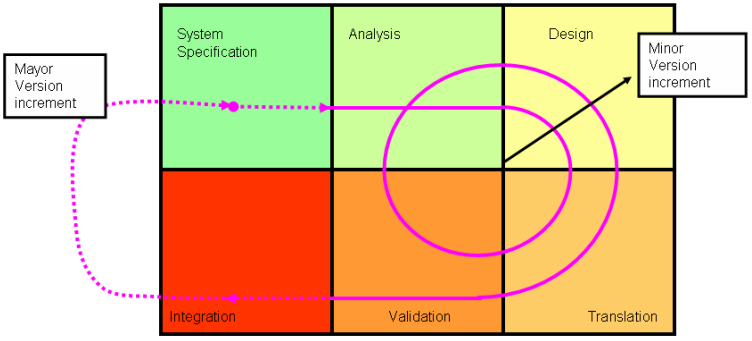
\includegraphics[width=0.9\linewidth]{figures/6Q.png}
\end{figure}
%
\subsection{Singleton}
\begin{lstlisting}[style=Cpp]
class Singleton {
public:
  static Singleton& getInstance() {
    static Singleton instance;
    return instance;
}
private:
  // Private constructor and desctructor
  Singleton() {};
  Singleton(const Singleton&) {};
  void operator=(const Singleton&) {};
};

int main() {
  Singleton::getInstace().doSomething();
}
\end{lstlisting}
%
\subsection{Concept of 5 layers}
\begin{enumerate}
    \item \textbf{Application :} contrôle de l'application
    \item \textbf{Middleware :} éléments de communication
    \item \textbf{RTOS :} OS temps réel
    \item \textbf{Board :} mise en miroir du hardware
    \item \textbf{HAL :} abstraction des périphériques hardware
    \item \textbf{Common :} paquet virtuel du système
\end{enumerate}
\begin{figure}[H]
    \centering
    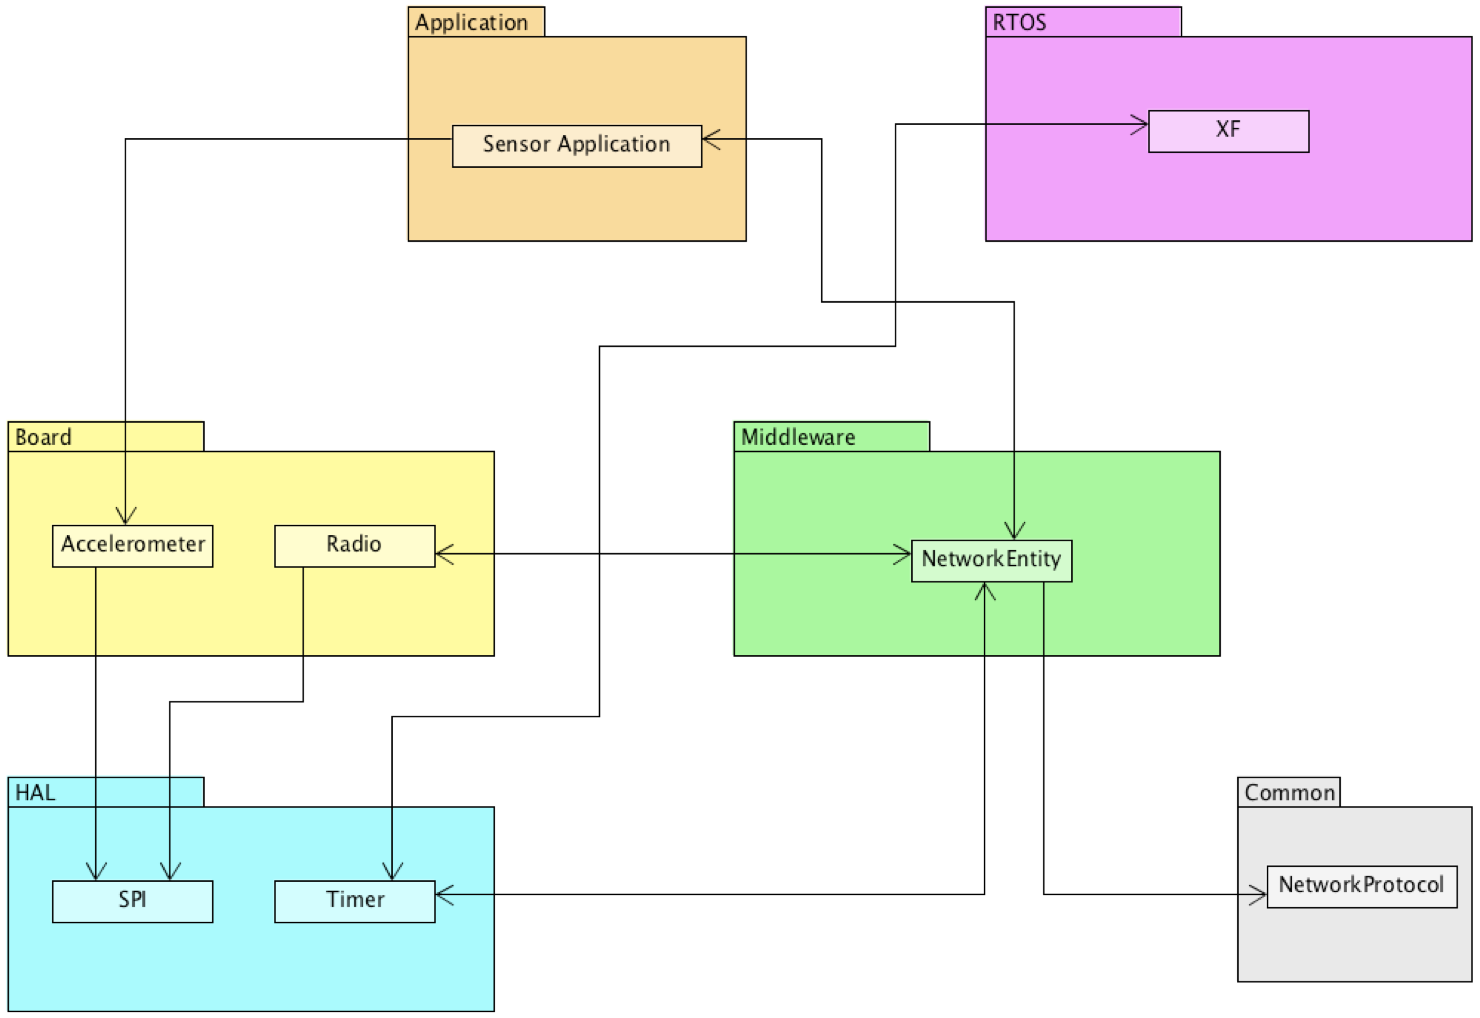
\includegraphics[width=0.8\linewidth]{figures/5_layers.png}
\end{figure}
%
\subsection{Factory}
\begin{figure}[H]
    \centering
    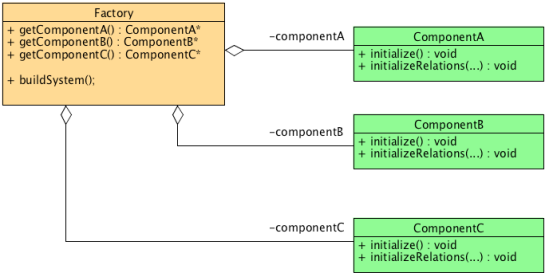
\includegraphics[width=7.00cm]{figures/factory.png}
\end{figure}
Dans \verb+buildSystem()+ :
\begin{enumerate}
    \item \verb!create!
    \item \verb!initialize!
    \item \verb!initializeRelations! quand tous les \verb!create! et \verb!initialize! sont faits
\end{enumerate}
%
\subsection{Observateur}
Dérivé du pattern \textit{Observer}.
\begin{figure}[H]
    \centering
    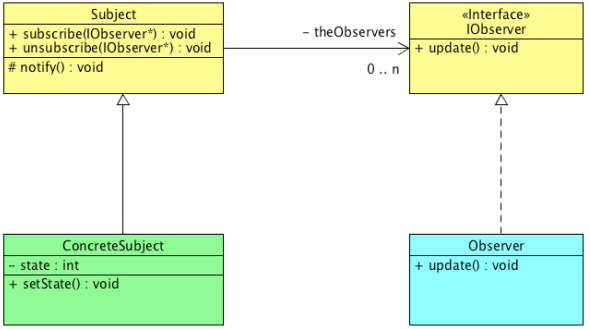
\includegraphics[width=7.00cm]{figures/observer.png}
\end{figure}
%
\subsection{Interface SAP (Service Access Point)}
\begin{figure}[H]
    \centering
    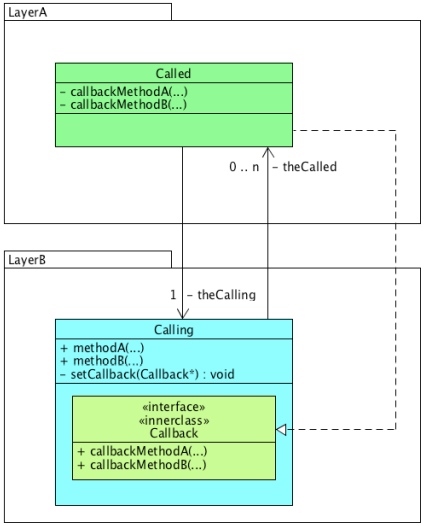
\includegraphics[width=7.00cm]{figures/SAP_1.png}
\end{figure}
\begin{figure}[H]
    \centering
    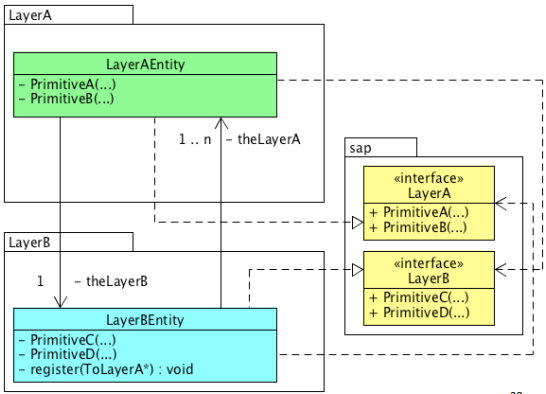
\includegraphics[width=7.00cm]{figures/SAP_2.png}
\end{figure}
